% Options for packages loaded elsewhere
\PassOptionsToPackage{unicode}{hyperref}
\PassOptionsToPackage{hyphens}{url}
%
\documentclass[
  ignorenonframetext,
  usenames,
  dvipsnames]{beamer}
\usepackage{pgfpages}
\setbeamertemplate{caption}[numbered]
\setbeamertemplate{caption label separator}{: }
\setbeamercolor{caption name}{fg=normal text.fg}
\beamertemplatenavigationsymbolsempty
% Prevent slide breaks in the middle of a paragraph
\widowpenalties 1 10000
\raggedbottom
\setbeamertemplate{part page}{
  \centering
  \begin{beamercolorbox}[sep=16pt,center]{part title}
    \usebeamerfont{part title}\insertpart\par
  \end{beamercolorbox}
}
\setbeamertemplate{section page}{
  \centering
  \begin{beamercolorbox}[sep=12pt,center]{part title}
    \usebeamerfont{section title}\insertsection\par
  \end{beamercolorbox}
}
\setbeamertemplate{subsection page}{
  \centering
  \begin{beamercolorbox}[sep=8pt,center]{part title}
    \usebeamerfont{subsection title}\insertsubsection\par
  \end{beamercolorbox}
}
\AtBeginPart{
  \frame{\partpage}
}
\AtBeginSection{
  \ifbibliography
  \else
    \frame{\sectionpage}
  \fi
}
\AtBeginSubsection{
  \frame{\subsectionpage}
}
\usepackage{lmodern}
\usepackage{amsmath}
\usepackage{ifxetex,ifluatex}
\ifnum 0\ifxetex 1\fi\ifluatex 1\fi=0 % if pdftex
  \usepackage[T1]{fontenc}
  \usepackage[utf8]{inputenc}
  \usepackage{textcomp} % provide euro and other symbols
  \usepackage{amssymb}
\else % if luatex or xetex
  \usepackage{unicode-math}
  \defaultfontfeatures{Scale=MatchLowercase}
  \defaultfontfeatures[\rmfamily]{Ligatures=TeX,Scale=1}
\fi
% Use upquote if available, for straight quotes in verbatim environments
\IfFileExists{upquote.sty}{\usepackage{upquote}}{}
\IfFileExists{microtype.sty}{% use microtype if available
  \usepackage[]{microtype}
  \UseMicrotypeSet[protrusion]{basicmath} % disable protrusion for tt fonts
}{}
\makeatletter
\@ifundefined{KOMAClassName}{% if non-KOMA class
  \IfFileExists{parskip.sty}{%
    \usepackage{parskip}
  }{% else
    \setlength{\parindent}{0pt}
    \setlength{\parskip}{6pt plus 2pt minus 1pt}}
}{% if KOMA class
  \KOMAoptions{parskip=half}}
\makeatother
\usepackage{xcolor}
\IfFileExists{xurl.sty}{\usepackage{xurl}}{} % add URL line breaks if available
\IfFileExists{bookmark.sty}{\usepackage{bookmark}}{\usepackage{hyperref}}
\hypersetup{
  pdftitle={Diversity and Inclusion Report},
  pdfauthor={Dr.~Philippe De Brouwer},
  hidelinks,
  pdfcreator={LaTeX via pandoc}}
\urlstyle{same} % disable monospaced font for URLs
\newif\ifbibliography
\usepackage{graphicx}
\makeatletter
\def\maxwidth{\ifdim\Gin@nat@width>\linewidth\linewidth\else\Gin@nat@width\fi}
\def\maxheight{\ifdim\Gin@nat@height>\textheight\textheight\else\Gin@nat@height\fi}
\makeatother
% Scale images if necessary, so that they will not overflow the page
% margins by default, and it is still possible to overwrite the defaults
% using explicit options in \includegraphics[width, height, ...]{}
\setkeys{Gin}{width=\maxwidth,height=\maxheight,keepaspectratio}
% Set default figure placement to htbp
\makeatletter
\def\fps@figure{htbp}
\makeatother
\setlength{\emergencystretch}{3em} % prevent overfull lines
\providecommand{\tightlist}{%
  \setlength{\itemsep}{0pt}\setlength{\parskip}{0pt}}
\setcounter{secnumdepth}{-\maxdimen} % remove section numbering
\usetheme[progressbar=frametitle]{metropolis}
\usepackage{booktabs}
\usepackage{longtable}
\usepackage{array}
\usepackage{multirow}
\usepackage{wrapfig}
\usepackage{float}
\usepackage{colortbl}
\usepackage{pdflscape}
\usepackage{tabu}
\usepackage{threeparttable}
\usepackage{threeparttablex}
\usepackage[normalem]{ulem}
\usepackage{makecell}
\usepackage{xcolor}
\ifluatex
  \usepackage{selnolig}  % disable illegal ligatures
\fi
\newlength{\cslhangindent}
\setlength{\cslhangindent}{1.5em}
\newlength{\csllabelwidth}
\setlength{\csllabelwidth}{3em}
\newenvironment{CSLReferences}[2] % #1 hanging-ident, #2 entry spacing
 {% don't indent paragraphs
  \setlength{\parindent}{0pt}
  % turn on hanging indent if param 1 is 1
  \ifodd #1 \everypar{\setlength{\hangindent}{\cslhangindent}}\ignorespaces\fi
  % set entry spacing
  \ifnum #2 > 0
  \setlength{\parskip}{#2\baselineskip}
  \fi
 }%
 {}
\usepackage{calc}
\newcommand{\CSLBlock}[1]{#1\hfill\break}
\newcommand{\CSLLeftMargin}[1]{\parbox[t]{\csllabelwidth}{#1}}
\newcommand{\CSLRightInline}[1]{\parbox[t]{\linewidth - \csllabelwidth}{#1}\break}
\newcommand{\CSLIndent}[1]{\hspace{\cslhangindent}#1}

\title{Diversity and Inclusion Report}
\subtitle{This report uses randomly generated data and does not reflect
the situation in a perticular company.}
\author{Dr.~Philippe De Brouwer}
\date{23 April, 2021}

\begin{document}
\frame{\titlepage}
\begin{abstract}
This report informs about how diverse the team is and tries to indicate
potential areas of bias. This report cannot prove or disprove bias, it
can only direct the user to potential problems. Hence this report is in
the first place an invitation to think. Much like feedback from other
people is an invitation to think and not a diagnosis per se.
\end{abstract}

\begin{frame}{Table of Contents}
\protect\hypertarget{table-of-contents}{}
\tableofcontents[hideallsubsections]
\end{frame}

\hypertarget{the-particular-example-behind-this-demo-report}{%
\section{The Particular Example Behind this Demo
Report}\label{the-particular-example-behind-this-demo-report}}

\begin{frame}{The Particular Example Behind this Demo Report}
The data used for this report is randomly generated with the following
characteristics:

\begin{itemize}
\tightlist
\item
  team size: 400
\item
  percentage of females: 0.35
\item
  average male's salary / average female's salary: 1.035
\item
  no other biases are built in (so any other observations stem from
  random generation of data. This can be seen as ``despite no bias
  against citizenship by the manager, some pay-gaps will be different
  from one.'' This means that being unbiased is not necessarily the same
  as having equal outcomes.)
\end{itemize}

\begin{block}{Equitable outcomes are not the same as equal outcomes!}
\protect\hypertarget{equitable-outcomes-are-not-the-same-as-equal-outcomes}{}
\end{block}
\end{frame}

\hypertarget{overview}{%
\section{Overview}\label{overview}}

\begin{frame}{Findings (in order of importance)}
\protect\hypertarget{findings-in-order-of-importance}{}
\small

\begin{tabular}{r|l|>{\raggedright\arraybackslash}p{12em}|>{\raggedright\arraybackslash}p{12em}}
\hline
Nbr & Area & Finding & Suggestion\\
\hline
1 & Gender & Where we can calculate the paygap between females and non-females, we find that the females generally earn less in similar roles and similar grades. & Check the gender-paygap table and identify the grade/role combinations where an the paygap has most stars. Check if the salary differences are justified.\\
\hline
2 & Age & The team is predominantly younger than the surrounding population (Poland). & Consider hiring older people to balance. Focus on retention.\\
\hline
3 & Gender & The diversity is good in grade 1 and 2, but under par in grade 3 & Consider if females have barriers to apply to grade 3 jobs and remove the barriers.\\
\hline
4 & Gender & Males in Grade 2 seem to have been promoted faster. & Understand unconscious bias, coach everyone (and specially females), work on trust.\\
\hline
\end{tabular}
\end{frame}

\begin{frame}{Dashboard}
\protect\hypertarget{dashboard}{}
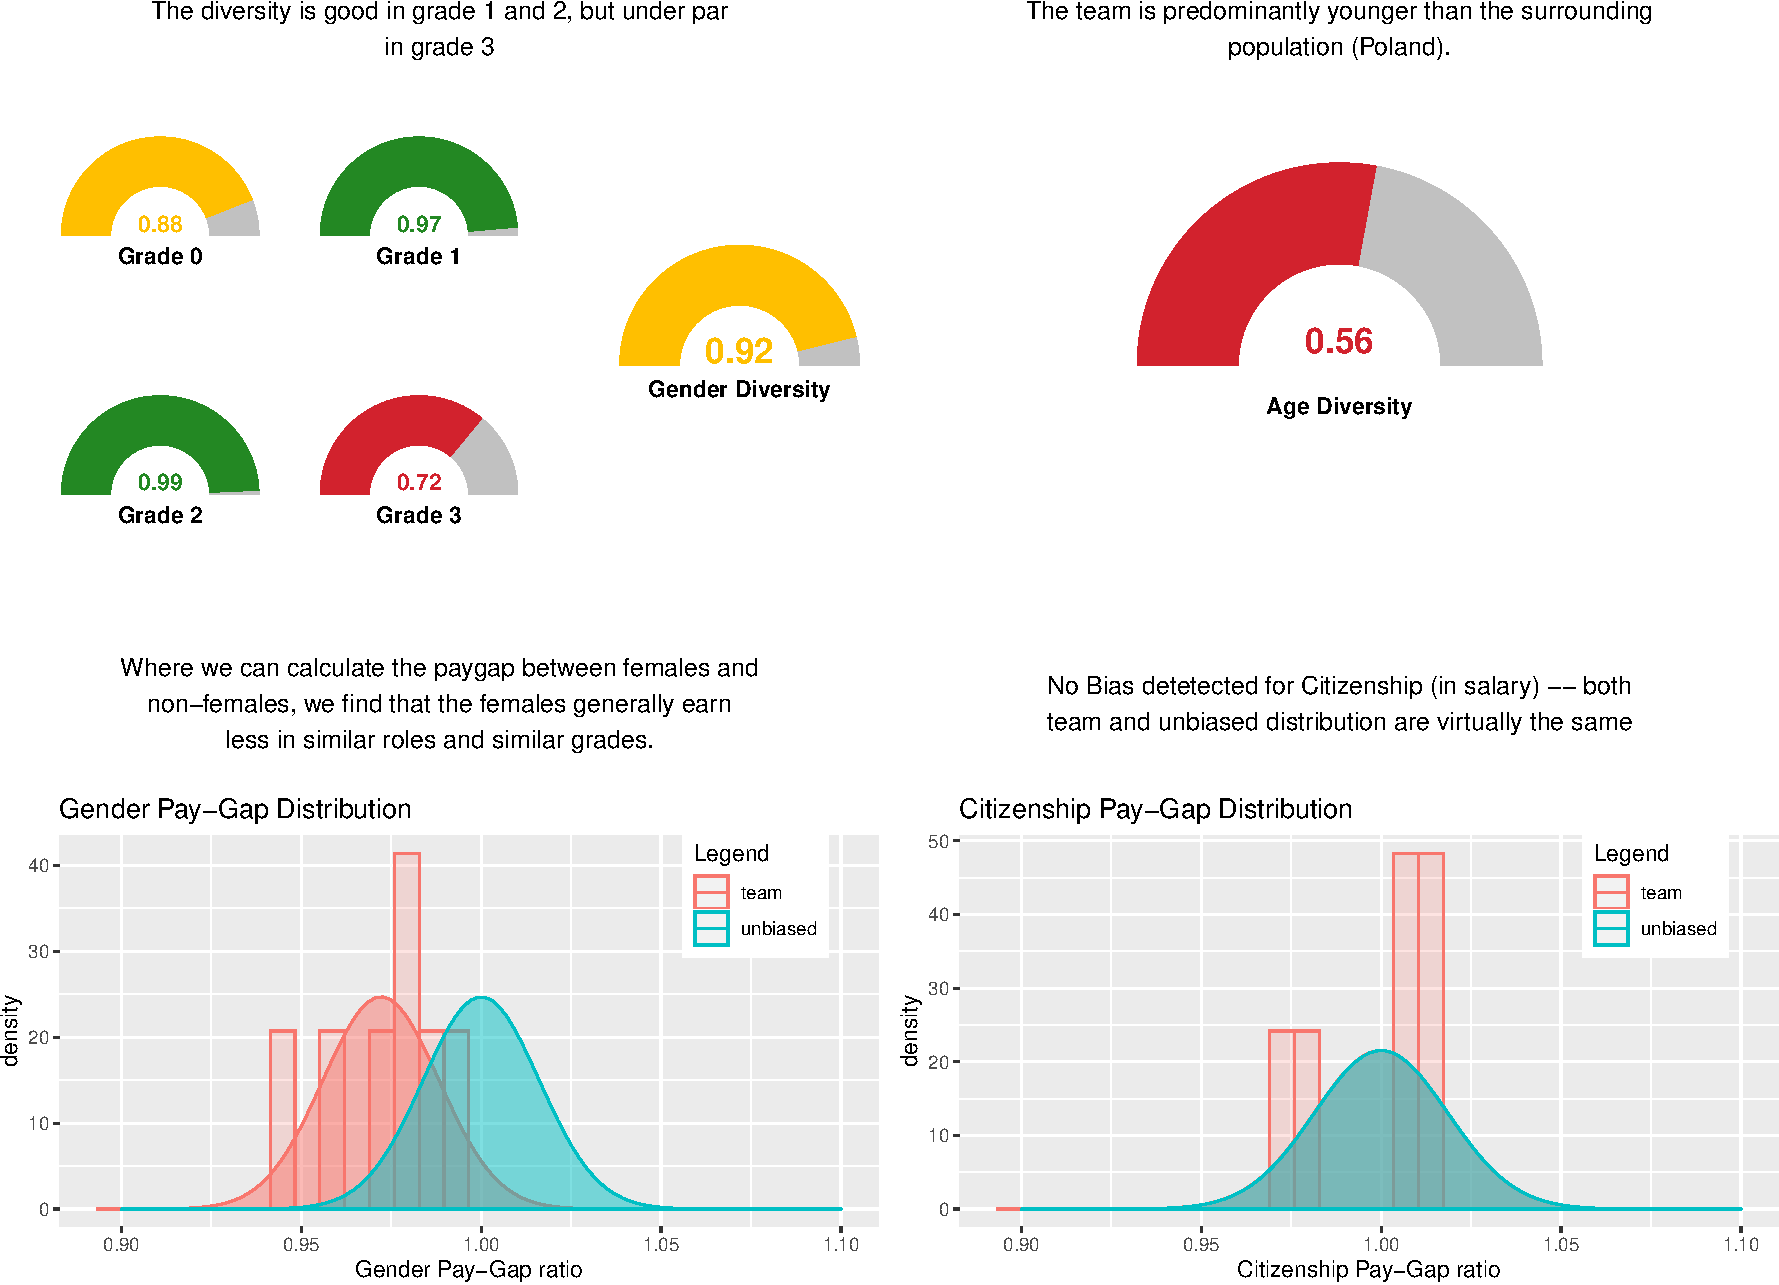
\includegraphics{team_slides_files/figure-beamer/dash-1.pdf}
\end{frame}

\hypertarget{diversity}{%
\section{Diversity}\label{diversity}}

\begin{frame}{Gender diversity per grade}
\protect\hypertarget{gender-diversity-per-grade}{}
\begin{figure}
\centering
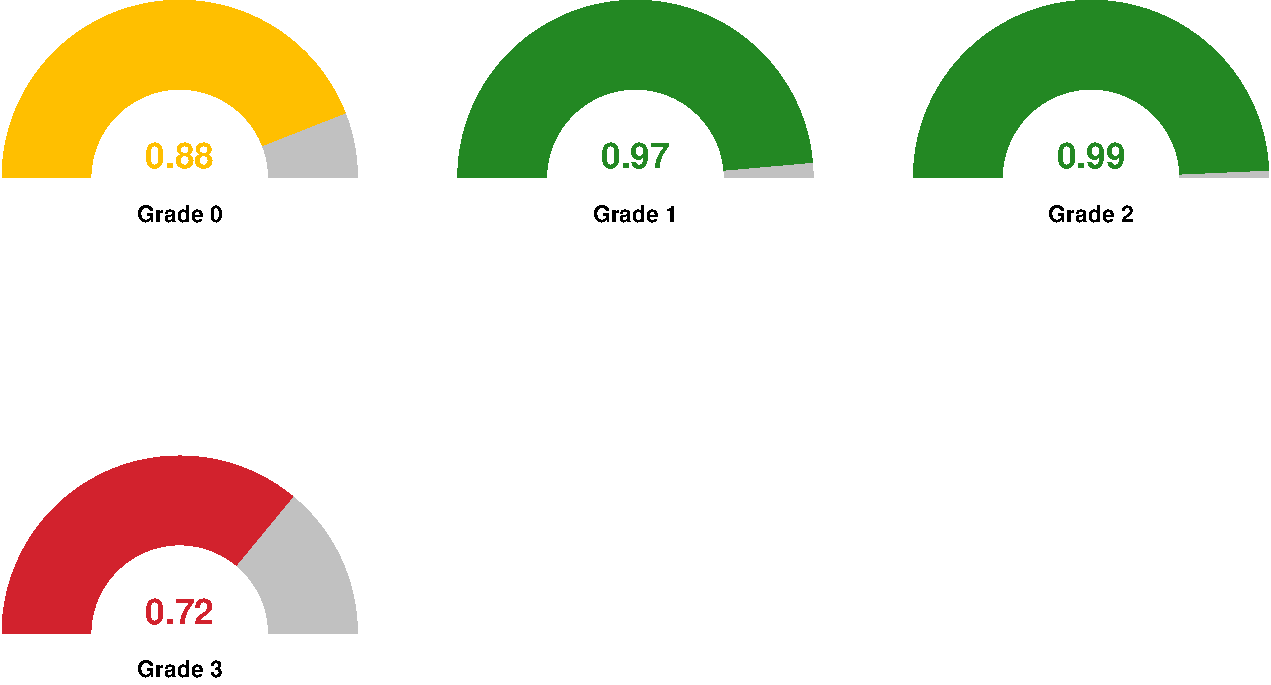
\includegraphics{team_slides_files/figure-beamer/unnamed-chunk-1-1.pdf}
\caption{The diversity of the team with respect to gender per
grade.\label{fig:gender-gauge}}
\end{figure}
\end{frame}

\begin{frame}{Age diversity}
\protect\hypertarget{age-diversity}{}
\begin{figure}
\centering
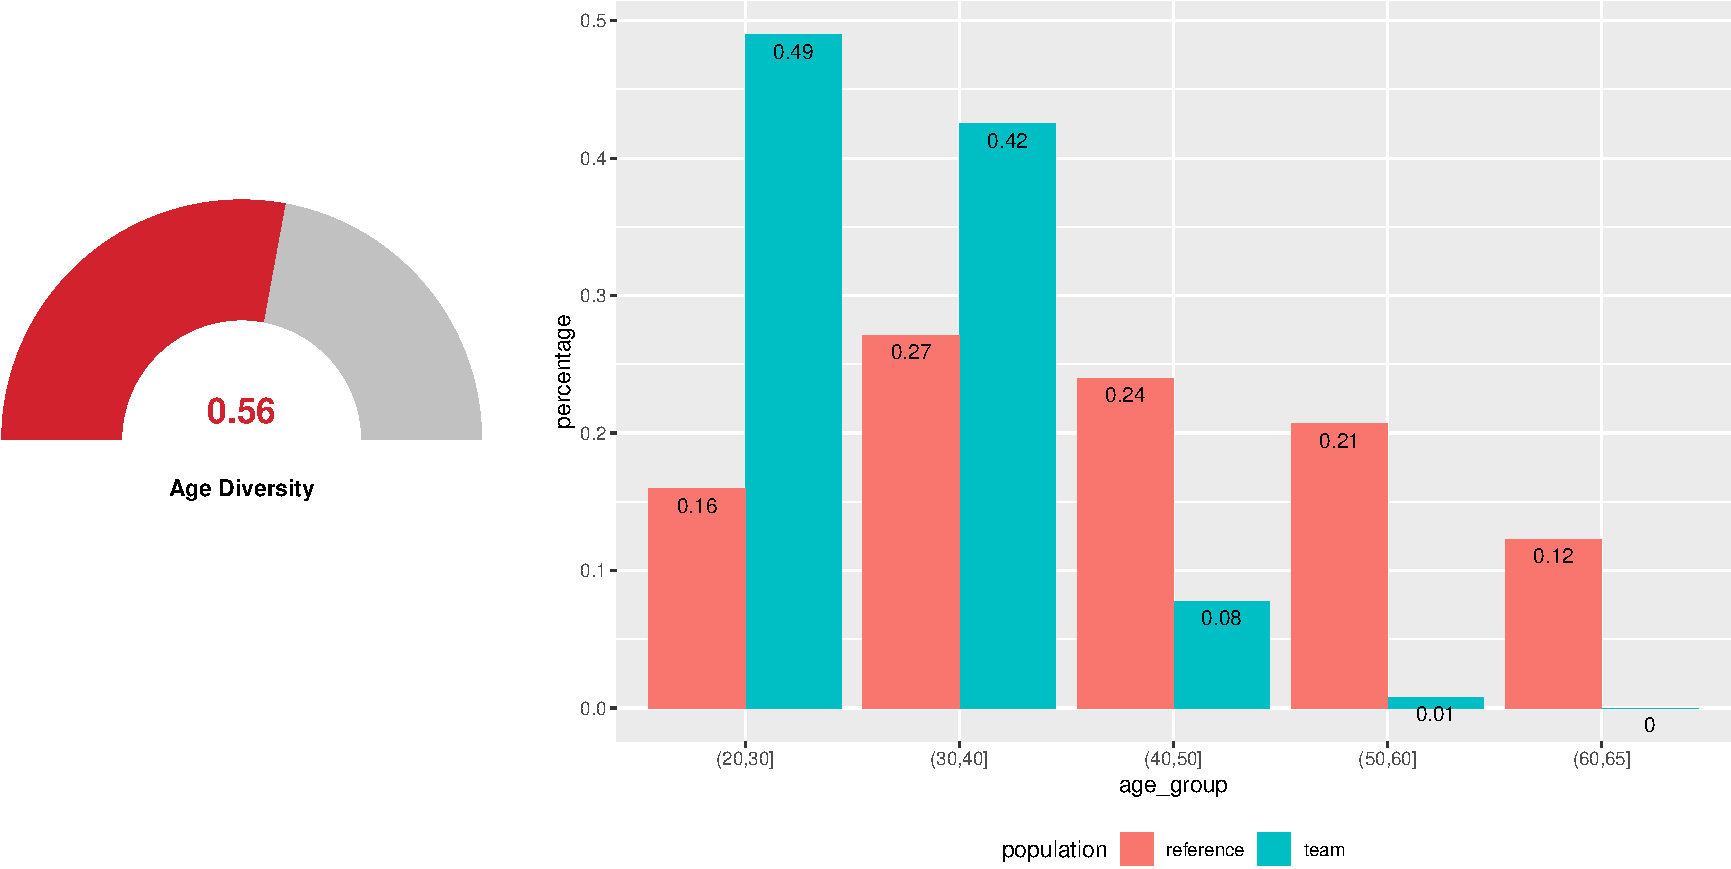
\includegraphics{team_slides_files/figure-beamer/ageism-1.pdf}
\caption{The diversity of the team with respect to age, assuming the age
distribution of the country as reference.\label{fig:ageism}}
\end{figure}
\end{frame}

\begin{frame}{Diversity in nationalities (1/2)}
\protect\hypertarget{diversity-in-nationalities-12}{}
\framesubtitle{Distribution for the team}

\begin{figure}
\centering
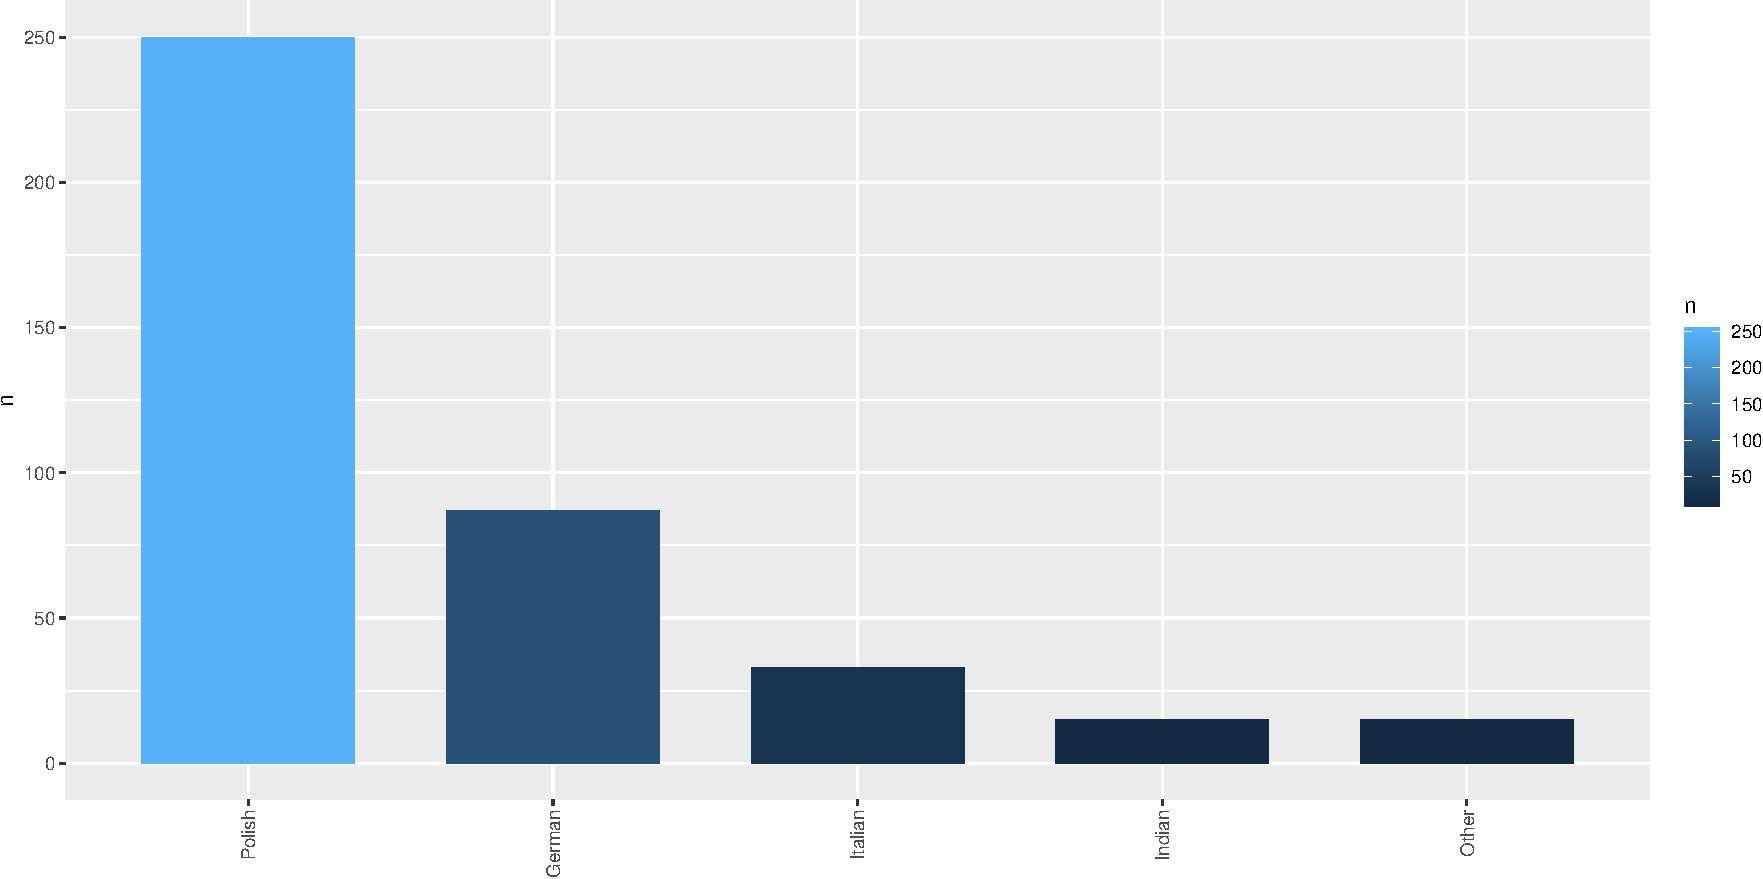
\includegraphics{team_slides_files/figure-beamer/nationalities-1.pdf}
\caption{The barplot for the nationalities in the team over all grades.}
\end{figure}
\end{frame}

\begin{frame}{Diversity in nationalities (2/2)}
\protect\hypertarget{diversity-in-nationalities-22}{}
\framesubtitle{Breakdown per Grade}

\begin{figure}
\centering
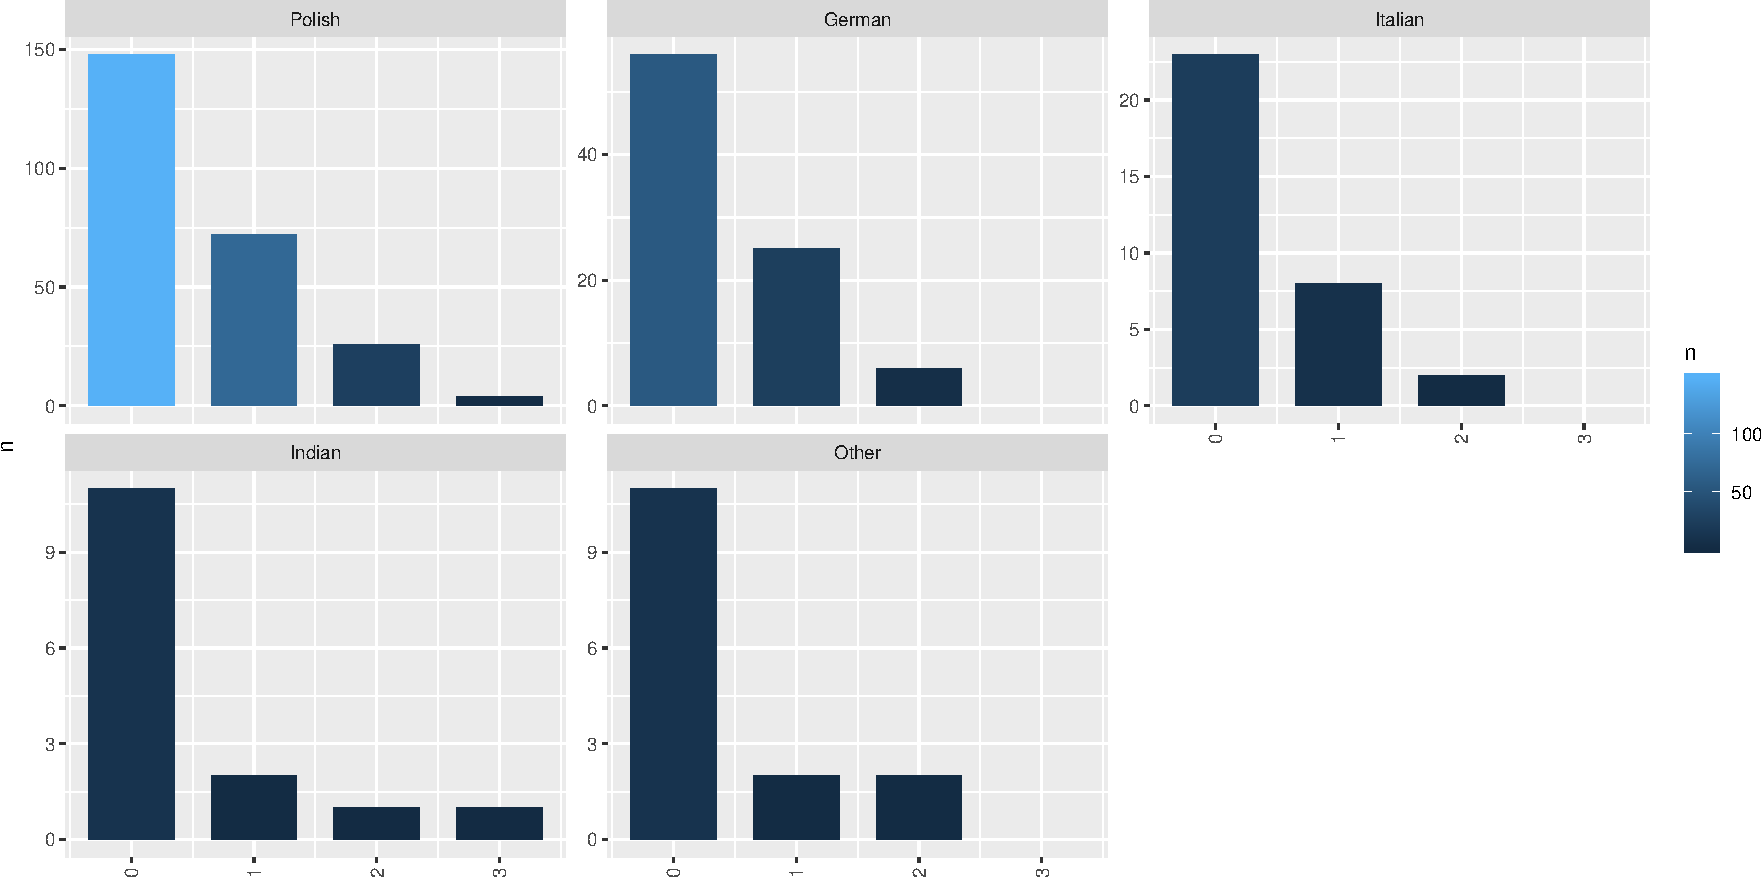
\includegraphics{team_slides_files/figure-beamer/nationalities2-1.pdf}
\caption{The breakdown of each grade per nationalitiy.}
\end{figure}
\end{frame}

\hypertarget{inclusion}{%
\section{Inclusion}\label{inclusion}}

\begin{frame}{The Gender PayGap}
\protect\hypertarget{the-gender-paygap}{}
\begin{table}

\caption{\label{tab:pg:gender}The paygap for gender (in terms of salary) as a ratio, along with  the confidence level that this paygap is significant alongside the control variable age.}
\centering
\resizebox{\linewidth}{!}{
\begin{tabular}[t]{>{}r|>{}l|>{}r|>{}r|>{}r|>{}r|>{}r|>{}r|>{}r|>{}r|>{}l}
\hline
\textbf{grade} & \textbf{jobID} & \textbf{sal\_F} & \textbf{sal\_oths} & \textbf{n\_F} & \textbf{n\_oths} & \textbf{med\_age\_F} & \textbf{med\_age\_o} & \textbf{paygap} & \textbf{p-value} & \textbf{conf.}\\
\hline
\cellcolor{BurntOrange}{\textcolor{black}{\textbf{\textbf{0}}}} & \cellcolor{BurntOrange}{\textcolor{black}{\textbf{sales}}} & \cellcolor{BurntOrange}{\textcolor{black}{\textbf{3,902}}} & \cellcolor{BurntOrange}{\textcolor{black}{\textbf{4,133}}} & \cellcolor{BurntOrange}{\textcolor{black}{\textbf{51}}} & \cellcolor{BurntOrange}{\textcolor{black}{\textbf{105}}} & \cellcolor{BurntOrange}{\textcolor{black}{\textbf{28.0}}} & \cellcolor{BurntOrange}{\textcolor{black}{\textbf{29.0}}} & \cellcolor{BurntOrange}{\textcolor{black}{\textbf{0.944}}} & \cellcolor{BurntOrange}{\textcolor{black}{\textbf{0.008647}}} & \cellcolor{BurntOrange}{\textcolor{black}{\textbf{**}}}\\
\hline
\cellcolor{red}{\textcolor{black}{\textbf{\textbf{2}}}} & \cellcolor{red}{\textcolor{black}{\textbf{sales}}} & \cellcolor{red}{\textcolor{black}{\textbf{17,971}}} & \cellcolor{red}{\textcolor{black}{\textbf{18,737}}} & \cellcolor{red}{\textcolor{black}{\textbf{12}}} & \cellcolor{red}{\textcolor{black}{\textbf{16}}} & \cellcolor{red}{\textcolor{black}{\textbf{34.5}}} & \cellcolor{red}{\textcolor{black}{\textbf{35.5}}} & \cellcolor{red}{\textcolor{black}{\textbf{0.959}}} & \cellcolor{red}{\textcolor{black}{\textbf{0.000670}}} & \cellcolor{red}{\textcolor{black}{\textbf{***}}}\\
\hline
\cellcolor{green}{\textcolor{black}{\textbf{\textbf{3}}}} & \cellcolor{green}{\textcolor{black}{\textbf{sales}}} & \cellcolor{green}{\textcolor{black}{\textbf{38,154}}} & \cellcolor{green}{\textcolor{black}{\textbf{39,326}}} & \cellcolor{green}{\textcolor{black}{\textbf{1}}} & \cellcolor{green}{\textcolor{black}{\textbf{3}}} & \cellcolor{green}{\textcolor{black}{\textbf{34.0}}} & \cellcolor{green}{\textcolor{black}{\textbf{39.0}}} & \cellcolor{green}{\textcolor{black}{\textbf{0.970}}} & \cellcolor{green}{\textcolor{black}{\textbf{0.500000}}} & \cellcolor{green}{\textcolor{black}{\textbf{}}}\\
\hline
\cellcolor{GreenYellow}{\textcolor{black}{\textbf{\textbf{1}}}} & \cellcolor{GreenYellow}{\textcolor{black}{\textbf{analytics}}} & \cellcolor{GreenYellow}{\textcolor{black}{\textbf{8,500}}} & \cellcolor{GreenYellow}{\textcolor{black}{\textbf{8,703}}} & \cellcolor{GreenYellow}{\textcolor{black}{\textbf{17}}} & \cellcolor{GreenYellow}{\textcolor{black}{\textbf{24}}} & \cellcolor{GreenYellow}{\textcolor{black}{\textbf{31.0}}} & \cellcolor{GreenYellow}{\textcolor{black}{\textbf{32.0}}} & \cellcolor{GreenYellow}{\textcolor{black}{\textbf{0.977}}} & \cellcolor{GreenYellow}{\textcolor{black}{\textbf{0.092868}}} & \cellcolor{GreenYellow}{\textcolor{black}{\textbf{.}}}\\
\hline
\cellcolor{GreenYellow}{\textcolor{black}{\textbf{\textbf{2}}}} & \cellcolor{GreenYellow}{\textcolor{black}{\textbf{analytics}}} & \cellcolor{GreenYellow}{\textcolor{black}{\textbf{18,022}}} & \cellcolor{GreenYellow}{\textcolor{black}{\textbf{18,443}}} & \cellcolor{GreenYellow}{\textcolor{black}{\textbf{4}}} & \cellcolor{GreenYellow}{\textcolor{black}{\textbf{5}}} & \cellcolor{GreenYellow}{\textcolor{black}{\textbf{37.0}}} & \cellcolor{GreenYellow}{\textcolor{black}{\textbf{36.0}}} & \cellcolor{GreenYellow}{\textcolor{black}{\textbf{0.977}}} & \cellcolor{GreenYellow}{\textcolor{black}{\textbf{0.063492}}} & \cellcolor{GreenYellow}{\textcolor{black}{\textbf{.}}}\\
\hline
\cellcolor{green}{\textcolor{black}{\textbf{\textbf{0}}}} & \cellcolor{green}{\textcolor{black}{\textbf{analytics}}} & \cellcolor{green}{\textcolor{black}{\textbf{4,177}}} & \cellcolor{green}{\textcolor{black}{\textbf{4,229}}} & \cellcolor{green}{\textcolor{black}{\textbf{24}}} & \cellcolor{green}{\textcolor{black}{\textbf{69}}} & \cellcolor{green}{\textcolor{black}{\textbf{27.0}}} & \cellcolor{green}{\textcolor{black}{\textbf{29.0}}} & \cellcolor{green}{\textcolor{black}{\textbf{0.988}}} & \cellcolor{green}{\textcolor{black}{\textbf{0.396839}}} & \cellcolor{green}{\textcolor{black}{\textbf{}}}\\
\hline
\cellcolor{green}{\textcolor{black}{\textbf{\textbf{1}}}} & \cellcolor{green}{\textcolor{black}{\textbf{sales}}} & \cellcolor{green}{\textcolor{black}{\textbf{8,625}}} & \cellcolor{green}{\textcolor{black}{\textbf{8,712}}} & \cellcolor{green}{\textcolor{black}{\textbf{27}}} & \cellcolor{green}{\textcolor{black}{\textbf{41}}} & \cellcolor{green}{\textcolor{black}{\textbf{32.0}}} & \cellcolor{green}{\textcolor{black}{\textbf{31.0}}} & \cellcolor{green}{\textcolor{black}{\textbf{0.990}}} & \cellcolor{green}{\textcolor{black}{\textbf{0.349614}}} & \cellcolor{green}{\textcolor{black}{\textbf{}}}\\
\hline
\cellcolor{Gray}{\textcolor{black}{\textbf{\textbf{3}}}} & \cellcolor{Gray}{\textcolor{black}{\textbf{analytics}}} & \cellcolor{Gray}{\textcolor{black}{\textbf{NA}}} & \cellcolor{Gray}{\textcolor{black}{\textbf{38,825}}} & \cellcolor{Gray}{\textcolor{black}{\textbf{0}}} & \cellcolor{Gray}{\textcolor{black}{\textbf{1}}} & \cellcolor{Gray}{\textcolor{black}{\textbf{NA}}} & \cellcolor{Gray}{\textcolor{black}{\textbf{43.0}}} & \cellcolor{Gray}{\textcolor{black}{\textbf{NA}}} & \cellcolor{Gray}{\textcolor{black}{\textbf{NA}}} & \cellcolor{Gray}{\textcolor{black}{\textbf{NA}}}\\
\hline
\end{tabular}}
\end{table}
\end{frame}

\begin{frame}{The Citizenship PayGap}
\protect\hypertarget{the-citizenship-paygap}{}
\begin{table}

\caption{\label{tab:pg:citizenship}The paygap for citizenship (in terms of salary) as a ratio, along with  the confidence level that this paygap is significant alongside the control variable age.}
\centering
\resizebox{\linewidth}{!}{
\begin{tabular}[t]{>{}r|>{}l|>{}r|>{}r|>{}r|>{}r|>{}r|>{}r|>{}r|>{}r|>{}l}
\hline
\textbf{grade} & \textbf{jobID} & \textbf{sal\_Polis} & \textbf{sal\_oths} & \textbf{n\_Polish} & \textbf{n\_oths} & \textbf{med\_age\_P} & \textbf{med\_age\_o} & \textbf{paygap} & \textbf{p-value} & \textbf{conf.}\\
\hline
\cellcolor{green}{\textcolor{black}{\textbf{\textbf{2}}}} & \cellcolor{green}{\textcolor{black}{\textbf{sales}}} & \cellcolor{green}{\textcolor{black}{\textbf{18,244}}} & \cellcolor{green}{\textcolor{black}{\textbf{18,700}}} & \cellcolor{green}{\textcolor{black}{\textbf{19}}} & \cellcolor{green}{\textcolor{black}{\textbf{9}}} & \cellcolor{green}{\textcolor{black}{\textbf{34.0}}} & \cellcolor{green}{\textcolor{black}{\textbf{36.0}}} & \cellcolor{green}{\textcolor{black}{\textbf{0.976}}} & \cellcolor{green}{\textcolor{black}{\textbf{0.307855}}} & \cellcolor{green}{\textcolor{black}{\textbf{}}}\\
\hline
\cellcolor{green}{\textcolor{black}{\textbf{\textbf{1}}}} & \cellcolor{green}{\textcolor{black}{\textbf{analytics}}} & \cellcolor{green}{\textcolor{black}{\textbf{8,560}}} & \cellcolor{green}{\textcolor{black}{\textbf{8,761}}} & \cellcolor{green}{\textcolor{black}{\textbf{26}}} & \cellcolor{green}{\textcolor{black}{\textbf{15}}} & \cellcolor{green}{\textcolor{black}{\textbf{32.5}}} & \cellcolor{green}{\textcolor{black}{\textbf{30.0}}} & \cellcolor{green}{\textcolor{black}{\textbf{0.977}}} & \cellcolor{green}{\textcolor{black}{\textbf{0.694702}}} & \cellcolor{green}{\textcolor{black}{\textbf{}}}\\
\hline
\cellcolor{green}{\textcolor{black}{\textbf{\textbf{0}}}} & \cellcolor{green}{\textcolor{black}{\textbf{analytics}}} & \cellcolor{green}{\textcolor{black}{\textbf{4,227}}} & \cellcolor{green}{\textcolor{black}{\textbf{4,193}}} & \cellcolor{green}{\textcolor{black}{\textbf{56}}} & \cellcolor{green}{\textcolor{black}{\textbf{37}}} & \cellcolor{green}{\textcolor{black}{\textbf{28.5}}} & \cellcolor{green}{\textcolor{black}{\textbf{28.0}}} & \cellcolor{green}{\textcolor{black}{\textbf{1.008}}} & \cellcolor{green}{\textcolor{black}{\textbf{0.275245}}} & \cellcolor{green}{\textcolor{black}{\textbf{}}}\\
\hline
\cellcolor{green}{\textcolor{black}{\textbf{\textbf{0}}}} & \cellcolor{green}{\textcolor{black}{\textbf{sales}}} & \cellcolor{green}{\textcolor{black}{\textbf{4,078}}} & \cellcolor{green}{\textcolor{black}{\textbf{4,042}}} & \cellcolor{green}{\textcolor{black}{\textbf{92}}} & \cellcolor{green}{\textcolor{black}{\textbf{64}}} & \cellcolor{green}{\textcolor{black}{\textbf{27.0}}} & \cellcolor{green}{\textcolor{black}{\textbf{29.0}}} & \cellcolor{green}{\textcolor{black}{\textbf{1.009}}} & \cellcolor{green}{\textcolor{black}{\textbf{0.664176}}} & \cellcolor{green}{\textcolor{black}{\textbf{}}}\\
\hline
\cellcolor{green}{\textcolor{black}{\textbf{\textbf{2}}}} & \cellcolor{green}{\textcolor{black}{\textbf{analytics}}} & \cellcolor{green}{\textcolor{black}{\textbf{18,207}}} & \cellcolor{green}{\textcolor{black}{\textbf{17,947}}} & \cellcolor{green}{\textcolor{black}{\textbf{7}}} & \cellcolor{green}{\textcolor{black}{\textbf{2}}} & \cellcolor{green}{\textcolor{black}{\textbf{35.0}}} & \cellcolor{green}{\textcolor{black}{\textbf{39.0}}} & \cellcolor{green}{\textcolor{black}{\textbf{1.014}}} & \cellcolor{green}{\textcolor{black}{\textbf{0.888889}}} & \cellcolor{green}{\textcolor{black}{\textbf{}}}\\
\hline
\cellcolor{green}{\textcolor{black}{\textbf{\textbf{1}}}} & \cellcolor{green}{\textcolor{black}{\textbf{sales}}} & \cellcolor{green}{\textcolor{black}{\textbf{8,702}}} & \cellcolor{green}{\textcolor{black}{\textbf{8,569}}} & \cellcolor{green}{\textcolor{black}{\textbf{46}}} & \cellcolor{green}{\textcolor{black}{\textbf{22}}} & \cellcolor{green}{\textcolor{black}{\textbf{32.5}}} & \cellcolor{green}{\textcolor{black}{\textbf{30.5}}} & \cellcolor{green}{\textcolor{black}{\textbf{1.016}}} & \cellcolor{green}{\textcolor{black}{\textbf{0.553660}}} & \cellcolor{green}{\textcolor{black}{\textbf{}}}\\
\hline
\cellcolor{Gray}{\textcolor{black}{\textbf{\textbf{3}}}} & \cellcolor{Gray}{\textcolor{black}{\textbf{sales}}} & \cellcolor{Gray}{\textcolor{black}{\textbf{39,035}}} & \cellcolor{Gray}{\textcolor{black}{\textbf{NA}}} & \cellcolor{Gray}{\textcolor{black}{\textbf{4}}} & \cellcolor{Gray}{\textcolor{black}{\textbf{0}}} & \cellcolor{Gray}{\textcolor{black}{\textbf{37.0}}} & \cellcolor{Gray}{\textcolor{black}{\textbf{NA}}} & \cellcolor{Gray}{\textcolor{black}{\textbf{NA}}} & \cellcolor{Gray}{\textcolor{black}{\textbf{NA}}} & \cellcolor{Gray}{\textcolor{black}{\textbf{NA}}}\\
\hline
\cellcolor{Gray}{\textcolor{black}{\textbf{\textbf{3}}}} & \cellcolor{Gray}{\textcolor{black}{\textbf{analytics}}} & \cellcolor{Gray}{\textcolor{black}{\textbf{NA}}} & \cellcolor{Gray}{\textcolor{black}{\textbf{38,825}}} & \cellcolor{Gray}{\textcolor{black}{\textbf{0}}} & \cellcolor{Gray}{\textcolor{black}{\textbf{1}}} & \cellcolor{Gray}{\textcolor{black}{\textbf{NA}}} & \cellcolor{Gray}{\textcolor{black}{\textbf{43.0}}} & \cellcolor{Gray}{\textcolor{black}{\textbf{NA}}} & \cellcolor{Gray}{\textcolor{black}{\textbf{NA}}} & \cellcolor{Gray}{\textcolor{black}{\textbf{NA}}}\\
\hline
\end{tabular}}
\end{table}
\end{frame}

\begin{frame}{The Age Paygap}
\protect\hypertarget{the-age-paygap}{}
\begin{table}

\caption{\label{tab:pg:age}The paygap for age (in terms of salary) as a ratio, along with  the confidence level that this paygap is significant alongside the control variable age.}
\centering
\resizebox{\linewidth}{!}{
\begin{tabular}[t]{>{}r|>{}l|>{}r|>{}r|>{}r|>{}r|>{}r|>{}r|>{}r|>{}r|>{}l}
\hline
\textbf{grade} & \textbf{jobID} & \textbf{sal\_L} & \textbf{sal\_H} & \textbf{n\_L} & \textbf{n\_H} & \textbf{med\_age\_L} & \textbf{med\_age\_H} & \textbf{paygap} & \textbf{p-value} & \textbf{conf.}\\
\hline
\cellcolor{GreenYellow}{\textcolor{black}{\textbf{\textbf{1}}}} & \cellcolor{GreenYellow}{\textcolor{black}{\textbf{analytics}}} & \cellcolor{GreenYellow}{\textcolor{black}{\textbf{8,465}}} & \cellcolor{GreenYellow}{\textcolor{black}{\textbf{8,741}}} & \cellcolor{GreenYellow}{\textcolor{black}{\textbf{19}}} & \cellcolor{GreenYellow}{\textcolor{black}{\textbf{22}}} & \cellcolor{GreenYellow}{\textcolor{black}{\textbf{26.0}}} & \cellcolor{GreenYellow}{\textcolor{black}{\textbf{35.0}}} & \cellcolor{GreenYellow}{\textcolor{black}{\textbf{0.968}}} & \cellcolor{GreenYellow}{\textcolor{black}{\textbf{0.056311}}} & \cellcolor{GreenYellow}{\textcolor{black}{\textbf{.}}}\\
\hline
\cellcolor{green}{\textcolor{black}{\textbf{\textbf{2}}}} & \cellcolor{green}{\textcolor{black}{\textbf{sales}}} & \cellcolor{green}{\textcolor{black}{\textbf{18,130}}} & \cellcolor{green}{\textcolor{black}{\textbf{18,584}}} & \cellcolor{green}{\textcolor{black}{\textbf{14}}} & \cellcolor{green}{\textcolor{black}{\textbf{14}}} & \cellcolor{green}{\textcolor{black}{\textbf{32.0}}} & \cellcolor{green}{\textcolor{black}{\textbf{40.5}}} & \cellcolor{green}{\textcolor{black}{\textbf{0.976}}} & \cellcolor{green}{\textcolor{black}{\textbf{0.163552}}} & \cellcolor{green}{\textcolor{black}{\textbf{}}}\\
\hline
\cellcolor{green}{\textcolor{black}{\textbf{\textbf{3}}}} & \cellcolor{green}{\textcolor{black}{\textbf{sales}}} & \cellcolor{green}{\textcolor{black}{\textbf{38,740}}} & \cellcolor{green}{\textcolor{black}{\textbf{39,115}}} & \cellcolor{green}{\textcolor{black}{\textbf{2}}} & \cellcolor{green}{\textcolor{black}{\textbf{2}}} & \cellcolor{green}{\textcolor{black}{\textbf{34.5}}} & \cellcolor{green}{\textcolor{black}{\textbf{43.5}}} & \cellcolor{green}{\textcolor{black}{\textbf{0.990}}} & \cellcolor{green}{\textcolor{black}{\textbf{0.666667}}} & \cellcolor{green}{\textcolor{black}{\textbf{}}}\\
\hline
\cellcolor{green}{\textcolor{black}{\textbf{\textbf{0}}}} & \cellcolor{green}{\textcolor{black}{\textbf{analytics}}} & \cellcolor{green}{\textcolor{black}{\textbf{4,200}}} & \cellcolor{green}{\textcolor{black}{\textbf{4,221}}} & \cellcolor{green}{\textcolor{black}{\textbf{40}}} & \cellcolor{green}{\textcolor{black}{\textbf{53}}} & \cellcolor{green}{\textcolor{black}{\textbf{25.0}}} & \cellcolor{green}{\textcolor{black}{\textbf{32.0}}} & \cellcolor{green}{\textcolor{black}{\textbf{0.995}}} & \cellcolor{green}{\textcolor{black}{\textbf{0.568433}}} & \cellcolor{green}{\textcolor{black}{\textbf{}}}\\
\hline
\cellcolor{green}{\textcolor{black}{\textbf{\textbf{1}}}} & \cellcolor{green}{\textcolor{black}{\textbf{sales}}} & \cellcolor{green}{\textcolor{black}{\textbf{8,676}}} & \cellcolor{green}{\textcolor{black}{\textbf{8,609}}} & \cellcolor{green}{\textcolor{black}{\textbf{34}}} & \cellcolor{green}{\textcolor{black}{\textbf{34}}} & \cellcolor{green}{\textcolor{black}{\textbf{29.5}}} & \cellcolor{green}{\textcolor{black}{\textbf{36.0}}} & \cellcolor{green}{\textcolor{black}{\textbf{1.008}}} & \cellcolor{green}{\textcolor{black}{\textbf{0.692023}}} & \cellcolor{green}{\textcolor{black}{\textbf{}}}\\
\hline
\cellcolor{green}{\textcolor{black}{\textbf{\textbf{2}}}} & \cellcolor{green}{\textcolor{black}{\textbf{analytics}}} & \cellcolor{green}{\textcolor{black}{\textbf{18,270}}} & \cellcolor{green}{\textcolor{black}{\textbf{18,112}}} & \cellcolor{green}{\textcolor{black}{\textbf{4}}} & \cellcolor{green}{\textcolor{black}{\textbf{5}}} & \cellcolor{green}{\textcolor{black}{\textbf{32.0}}} & \cellcolor{green}{\textcolor{black}{\textbf{42.0}}} & \cellcolor{green}{\textcolor{black}{\textbf{1.009}}} & \cellcolor{green}{\textcolor{black}{\textbf{0.412698}}} & \cellcolor{green}{\textcolor{black}{\textbf{}}}\\
\hline
\cellcolor{green}{\textcolor{black}{\textbf{\textbf{0}}}} & \cellcolor{green}{\textcolor{black}{\textbf{sales}}} & \cellcolor{green}{\textcolor{black}{\textbf{4,106}}} & \cellcolor{green}{\textcolor{black}{\textbf{4,042}}} & \cellcolor{green}{\textcolor{black}{\textbf{72}}} & \cellcolor{green}{\textcolor{black}{\textbf{84}}} & \cellcolor{green}{\textcolor{black}{\textbf{24.0}}} & \cellcolor{green}{\textcolor{black}{\textbf{32.0}}} & \cellcolor{green}{\textcolor{black}{\textbf{1.016}}} & \cellcolor{green}{\textcolor{black}{\textbf{0.340726}}} & \cellcolor{green}{\textcolor{black}{\textbf{}}}\\
\hline
\cellcolor{Gray}{\textcolor{black}{\textbf{\textbf{3}}}} & \cellcolor{Gray}{\textcolor{black}{\textbf{analytics}}} & \cellcolor{Gray}{\textcolor{black}{\textbf{NA}}} & \cellcolor{Gray}{\textcolor{black}{\textbf{38,825}}} & \cellcolor{Gray}{\textcolor{black}{\textbf{0}}} & \cellcolor{Gray}{\textcolor{black}{\textbf{1}}} & \cellcolor{Gray}{\textcolor{black}{\textbf{NA}}} & \cellcolor{Gray}{\textcolor{black}{\textbf{43.0}}} & \cellcolor{Gray}{\textcolor{black}{\textbf{NA}}} & \cellcolor{Gray}{\textcolor{black}{\textbf{NA}}} & \cellcolor{Gray}{\textcolor{black}{\textbf{NA}}}\\
\hline
\end{tabular}}
\end{table}
\end{frame}

\begin{frame}{Time in firm paygap}
\protect\hypertarget{time-in-firm-paygap}{}
\begin{table}

\caption{\label{tab:pg:tenure_firm}The paygap for tenure firm (in terms of salary) as a ratio, along with  the confidence level that this paygap is significant alongside the control variable age.}
\centering
\resizebox{\linewidth}{!}{
\begin{tabular}[t]{>{}r|>{}l|>{}r|>{}r|>{}r|>{}r|>{}r|>{}r|>{}r|>{}r|>{}l}
\hline
\textbf{grade} & \textbf{jobID} & \textbf{sal\_L} & \textbf{sal\_H} & \textbf{n\_L} & \textbf{n\_H} & \textbf{med\_age\_L} & \textbf{med\_age\_H} & \textbf{paygap} & \textbf{p-value} & \textbf{conf.}\\
\hline
\cellcolor{GreenYellow}{\textcolor{black}{\textbf{\textbf{1}}}} & \cellcolor{GreenYellow}{\textcolor{black}{\textbf{sales}}} & \cellcolor{GreenYellow}{\textcolor{black}{\textbf{8,566}}} & \cellcolor{GreenYellow}{\textcolor{black}{\textbf{8,854}}} & \cellcolor{GreenYellow}{\textcolor{black}{\textbf{34}}} & \cellcolor{GreenYellow}{\textcolor{black}{\textbf{34}}} & \cellcolor{GreenYellow}{\textcolor{black}{\textbf{33.0}}} & \cellcolor{GreenYellow}{\textcolor{black}{\textbf{31.0}}} & \cellcolor{GreenYellow}{\textcolor{black}{\textbf{0.968}}} & \cellcolor{GreenYellow}{\textcolor{black}{\textbf{0.078323}}} & \cellcolor{GreenYellow}{\textcolor{black}{\textbf{.}}}\\
\hline
\cellcolor{green}{\textcolor{black}{\textbf{\textbf{0}}}} & \cellcolor{green}{\textcolor{black}{\textbf{sales}}} & \cellcolor{green}{\textcolor{black}{\textbf{4,040}}} & \cellcolor{green}{\textcolor{black}{\textbf{4,125}}} & \cellcolor{green}{\textcolor{black}{\textbf{78}}} & \cellcolor{green}{\textcolor{black}{\textbf{78}}} & \cellcolor{green}{\textcolor{black}{\textbf{28.0}}} & \cellcolor{green}{\textcolor{black}{\textbf{28.0}}} & \cellcolor{green}{\textcolor{black}{\textbf{0.979}}} & \cellcolor{green}{\textcolor{black}{\textbf{0.614746}}} & \cellcolor{green}{\textcolor{black}{\textbf{}}}\\
\hline
\cellcolor{green}{\textcolor{black}{\textbf{\textbf{2}}}} & \cellcolor{green}{\textcolor{black}{\textbf{sales}}} & \cellcolor{green}{\textcolor{black}{\textbf{18,228}}} & \cellcolor{green}{\textcolor{black}{\textbf{18,535}}} & \cellcolor{green}{\textcolor{black}{\textbf{14}}} & \cellcolor{green}{\textcolor{black}{\textbf{14}}} & \cellcolor{green}{\textcolor{black}{\textbf{35.5}}} & \cellcolor{green}{\textcolor{black}{\textbf{35.0}}} & \cellcolor{green}{\textcolor{black}{\textbf{0.983}}} & \cellcolor{green}{\textcolor{black}{\textbf{0.874287}}} & \cellcolor{green}{\textcolor{black}{\textbf{}}}\\
\hline
\cellcolor{green}{\textcolor{black}{\textbf{\textbf{3}}}} & \cellcolor{green}{\textcolor{black}{\textbf{sales}}} & \cellcolor{green}{\textcolor{black}{\textbf{38,740}}} & \cellcolor{green}{\textcolor{black}{\textbf{39,115}}} & \cellcolor{green}{\textcolor{black}{\textbf{2}}} & \cellcolor{green}{\textcolor{black}{\textbf{2}}} & \cellcolor{green}{\textcolor{black}{\textbf{34.5}}} & \cellcolor{green}{\textcolor{black}{\textbf{43.5}}} & \cellcolor{green}{\textcolor{black}{\textbf{0.990}}} & \cellcolor{green}{\textcolor{black}{\textbf{0.666667}}} & \cellcolor{green}{\textcolor{black}{\textbf{}}}\\
\hline
\cellcolor{green}{\textcolor{black}{\textbf{\textbf{0}}}} & \cellcolor{green}{\textcolor{black}{\textbf{analytics}}} & \cellcolor{green}{\textcolor{black}{\textbf{4,237}}} & \cellcolor{green}{\textcolor{black}{\textbf{4,207}}} & \cellcolor{green}{\textcolor{black}{\textbf{46}}} & \cellcolor{green}{\textcolor{black}{\textbf{47}}} & \cellcolor{green}{\textcolor{black}{\textbf{28.0}}} & \cellcolor{green}{\textcolor{black}{\textbf{28.0}}} & \cellcolor{green}{\textcolor{black}{\textbf{1.007}}} & \cellcolor{green}{\textcolor{black}{\textbf{0.865754}}} & \cellcolor{green}{\textcolor{black}{\textbf{}}}\\
\hline
\cellcolor{green}{\textcolor{black}{\textbf{\textbf{2}}}} & \cellcolor{green}{\textcolor{black}{\textbf{analytics}}} & \cellcolor{green}{\textcolor{black}{\textbf{18,270}}} & \cellcolor{green}{\textcolor{black}{\textbf{18,112}}} & \cellcolor{green}{\textcolor{black}{\textbf{4}}} & \cellcolor{green}{\textcolor{black}{\textbf{5}}} & \cellcolor{green}{\textcolor{black}{\textbf{32.0}}} & \cellcolor{green}{\textcolor{black}{\textbf{42.0}}} & \cellcolor{green}{\textcolor{black}{\textbf{1.009}}} & \cellcolor{green}{\textcolor{black}{\textbf{0.555556}}} & \cellcolor{green}{\textcolor{black}{\textbf{}}}\\
\hline
\cellcolor{green}{\textcolor{black}{\textbf{\textbf{1}}}} & \cellcolor{green}{\textcolor{black}{\textbf{analytics}}} & \cellcolor{green}{\textcolor{black}{\textbf{8,652}}} & \cellcolor{green}{\textcolor{black}{\textbf{8,495}}} & \cellcolor{green}{\textcolor{black}{\textbf{20}}} & \cellcolor{green}{\textcolor{black}{\textbf{21}}} & \cellcolor{green}{\textcolor{black}{\textbf{33.5}}} & \cellcolor{green}{\textcolor{black}{\textbf{30.0}}} & \cellcolor{green}{\textcolor{black}{\textbf{1.018}}} & \cellcolor{green}{\textcolor{black}{\textbf{0.705278}}} & \cellcolor{green}{\textcolor{black}{\textbf{}}}\\
\hline
\cellcolor{Gray}{\textcolor{black}{\textbf{\textbf{3}}}} & \cellcolor{Gray}{\textcolor{black}{\textbf{analytics}}} & \cellcolor{Gray}{\textcolor{black}{\textbf{NA}}} & \cellcolor{Gray}{\textcolor{black}{\textbf{38,825}}} & \cellcolor{Gray}{\textcolor{black}{\textbf{0}}} & \cellcolor{Gray}{\textcolor{black}{\textbf{1}}} & \cellcolor{Gray}{\textcolor{black}{\textbf{NA}}} & \cellcolor{Gray}{\textcolor{black}{\textbf{43.0}}} & \cellcolor{Gray}{\textcolor{black}{\textbf{NA}}} & \cellcolor{Gray}{\textcolor{black}{\textbf{NA}}} & \cellcolor{Gray}{\textcolor{black}{\textbf{NA}}}\\
\hline
\end{tabular}}
\end{table}
\end{frame}

\begin{frame}{Job Changes per Year per Gender}
\protect\hypertarget{job-changes-per-year-per-gender}{}
\begin{figure}
\centering
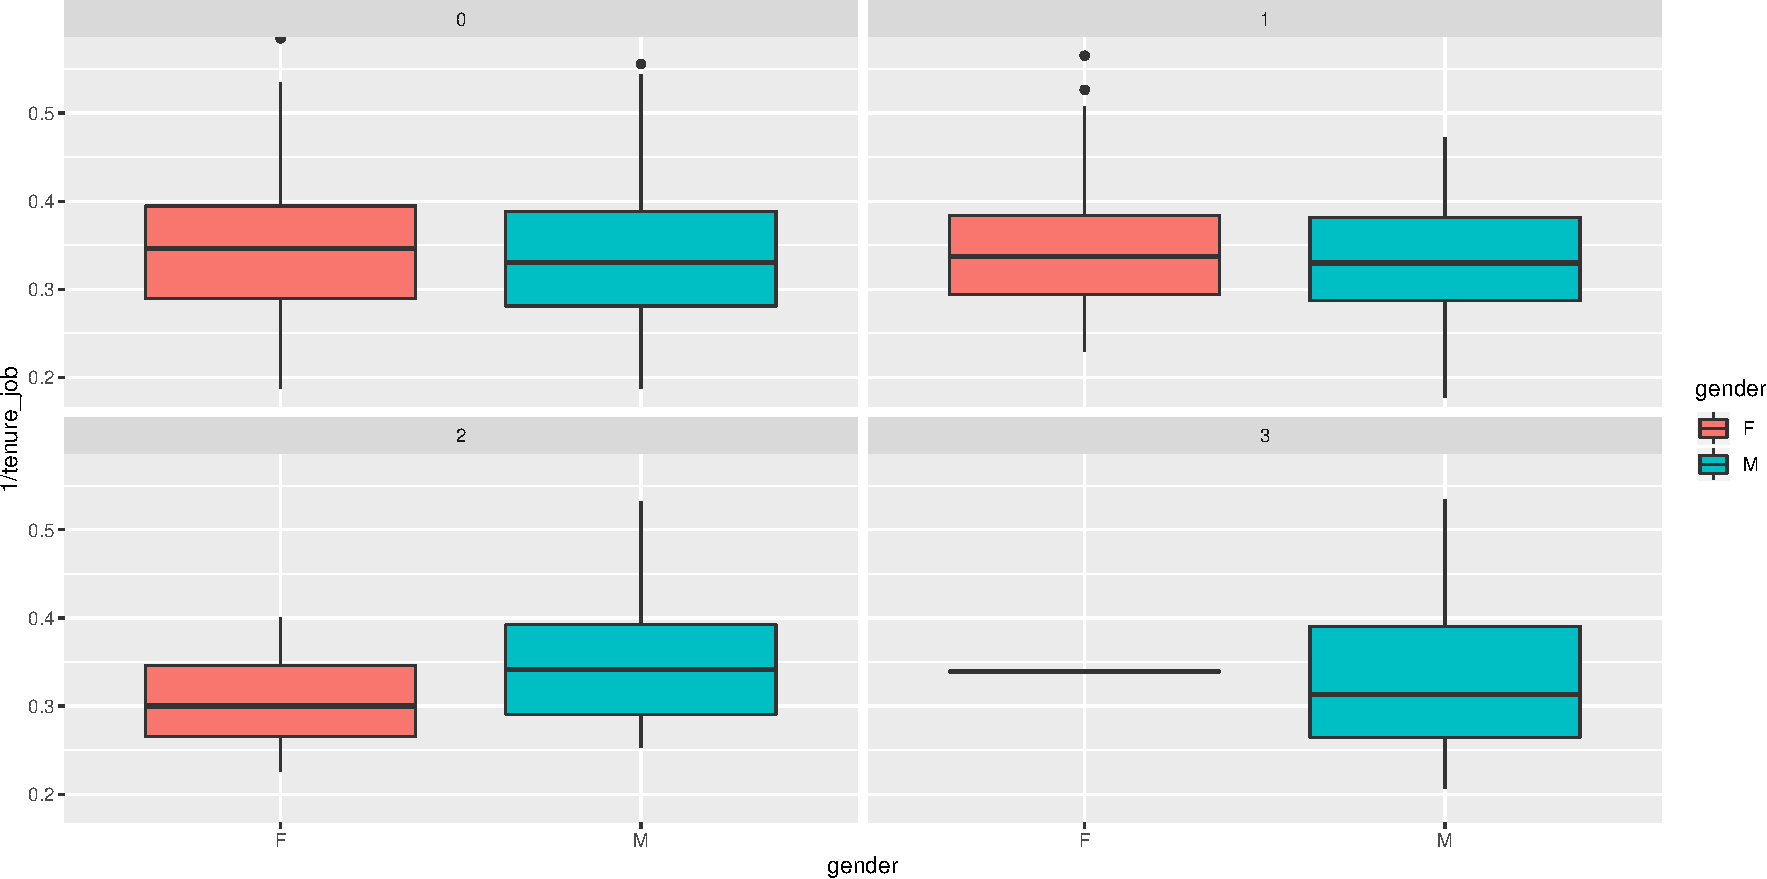
\includegraphics{team_slides_files/figure-beamer/TenureJob-1.pdf}
\caption{Job changes per year indicate mobility and risk taking. They
are a good indication for promotion (see Figure
\ref{fig:prom_p_gender}).}
\end{figure}
\end{frame}

\begin{frame}{Promotions per Year per Gender}
\protect\hypertarget{promotions-per-year-per-gender}{}
\begin{figure}
\centering
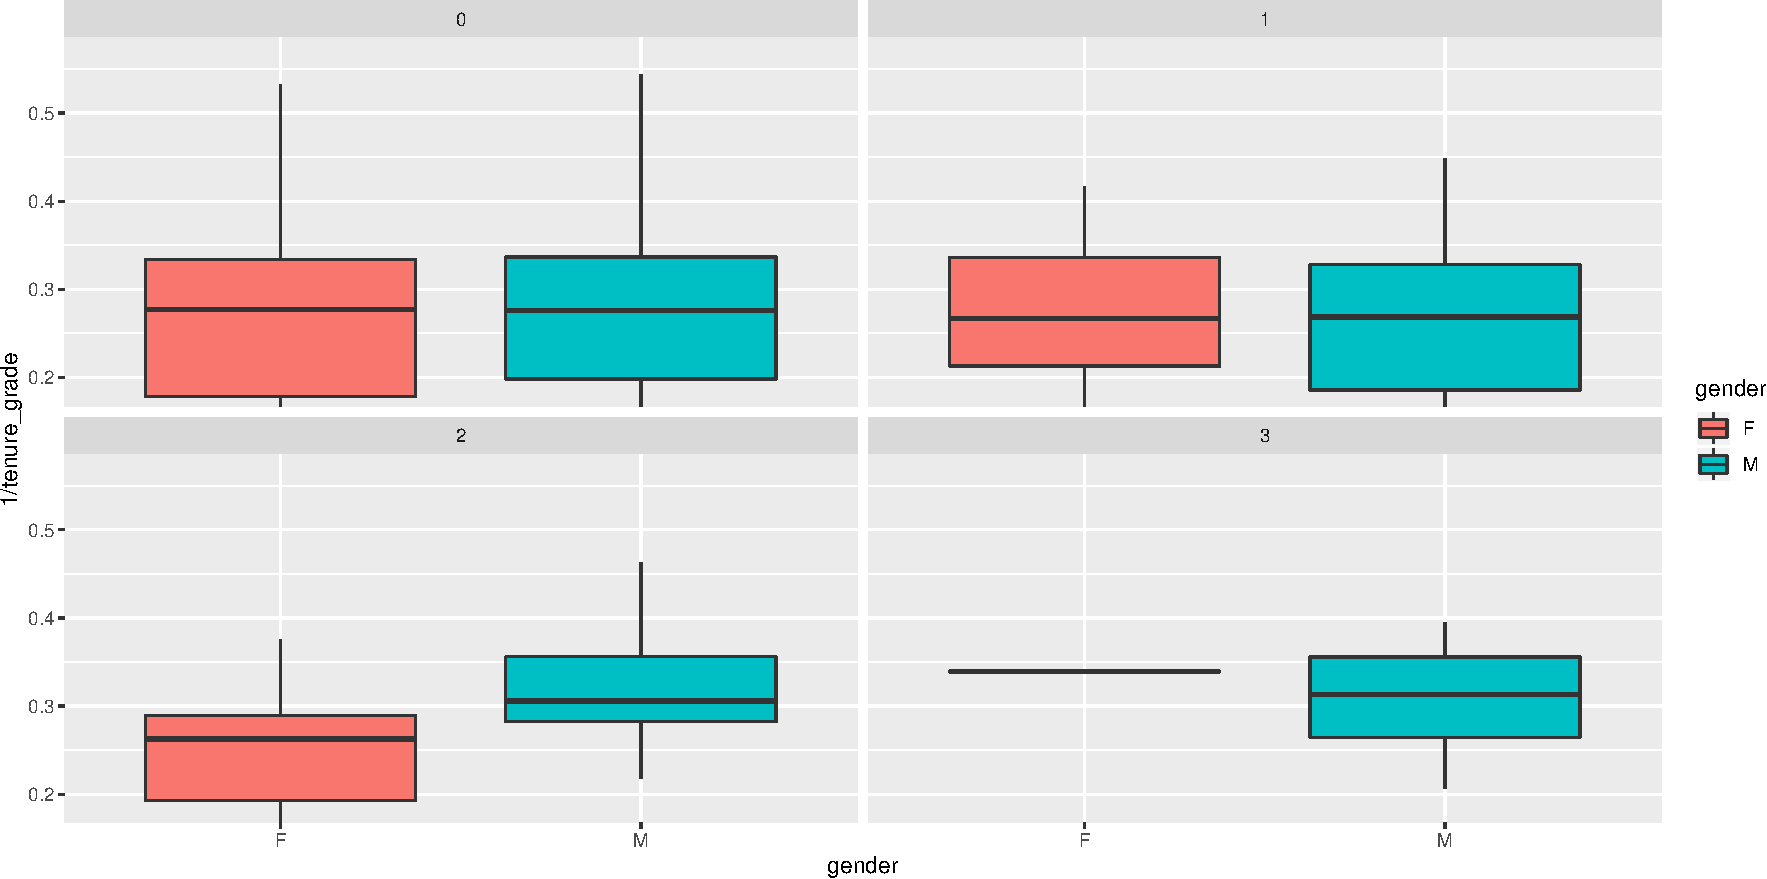
\includegraphics{team_slides_files/figure-beamer/TenureGrade-1.pdf}
\caption{The number of promotions per year can show if a gender is more
probable to be promoted.\label{fig:prom_p_gender}}
\end{figure}
\end{frame}

\hypertarget{conclusions}{%
\section{Conclusions}\label{conclusions}}

\begin{frame}{Conclusions}
\begin{tabular}{r|>{\raggedright\arraybackslash}p{22em}}
\hline
Nbr & Suggestion\\
\hline
0 & Learn more by reading e.g. "The Essentials of Diversification \& Inclusion", Dabrowska (2019)\\
\hline
1 & Check the gender-paygap table and identify the grade/role combinations where an the paygap has most stars. Check if the salary differences are justified.\\
\hline
2 & Consider hiring older people to balance. Focus on retention.\\
\hline
3 & Consider if females have barriers to apply to grade 3 jobs and remove the barriers.\\
\hline
4 & Understand unconscious bias, coach everyone (and specially females), work on trust.\\
\hline
\end{tabular}
\end{frame}

\hypertarget{appendices}{%
\section{Appendices}\label{appendices}}

\begin{frame}[fragile]{Legend Paygap}
\protect\hypertarget{legend-paygap}{}
\begin{itemize}
\tightlist
\item
  \texttt{paygap} = the ratio of median salaries of one group divided by
  the median of the salaries of the other group
\item
  \colorbox{Gray}{`NA`} = numbers are too small, please look at
  individuals;
\item
  \colorbox{green}{nothing} = no bias detectable;
\item
  \colorbox{GreenYellow}{`.`} = maybe there is some bias, but the
  numbers are low, check individuals;
\item
  \colorbox{Yellow}{`*`} = you should check for bias;
\item
  \colorbox{BurntOrange}{`**`} = bias is probably there;
\item
  \colorbox{red}{`***`} = most certainly there is bias
\end{itemize}

So, there will be more stars if the probability of a bias is higher:
this can be due to a higher bias and/or due to a larger sample size.
\end{frame}

\begin{frame}[fragile]{Legend: Paygap Column Headers}
\protect\hypertarget{legend-paygap-column-headers}{}
\small

\begin{itemize}
\tightlist
\item
  \texttt{grade} = the salary grade as used in the company
\item
  \texttt{jobID} = a unique identifier of the job category (can be
  abbreviated)
\item
  \texttt{sal\_F} = the median salary of the females (F)
\item
  \texttt{sal\_oth} = the median salary of the other groups (non F). The
  tool is open to use more than one gender.
\item
  \texttt{age\_F} = the median age of the females (or \texttt{age\_Pol}
  could be the median age of the team members with Polish citizenship)
\item
  \texttt{age\_oth} = the median age of the other groups take together
  (e.g.~the median age of non females)
\item
  \texttt{paygap} = the ratio of median salary earned by the selected
  group (e.g.~females) divided by the median of the other people. If
  this is lower than \(1\), then median female earns less than the
  median non-female.
\item
  \texttt{conf.} = the confidence level that this paygap is significant.
\end{itemize}
\end{frame}

\begin{frame}[shrink]{The Diversity Index (1/2)}
\protect\hypertarget{the-diversity-index-12}{}
We express diversity as a number between zero and one. Our calculation
is based on De Brouwer (2020) and more in particular section 36.3.1
``The Business Case: a Diversity Dashboard'\,'. Details can be found in
the book. The method is:

\begin{itemize}
\tightlist
\item
  The diversity is \(0\) if only one of the groups is present, and is
  \(1\) if both groups are equitably present.
\item
  This calculation is similar to the established concept of entropy in
  physics.
\item
  More than two categories can be used (e.g.~one is not limited to two
  genders)
\item
  We calibrate the probabilities so that they show maximum entropy (or
  diversity) for the percentages that naturally occur (see next slide).
\end{itemize}
\end{frame}

\begin{frame}{The Diversity Index (2/2)}
\protect\hypertarget{the-diversity-index-22}{}
\begin{figure}
\centering
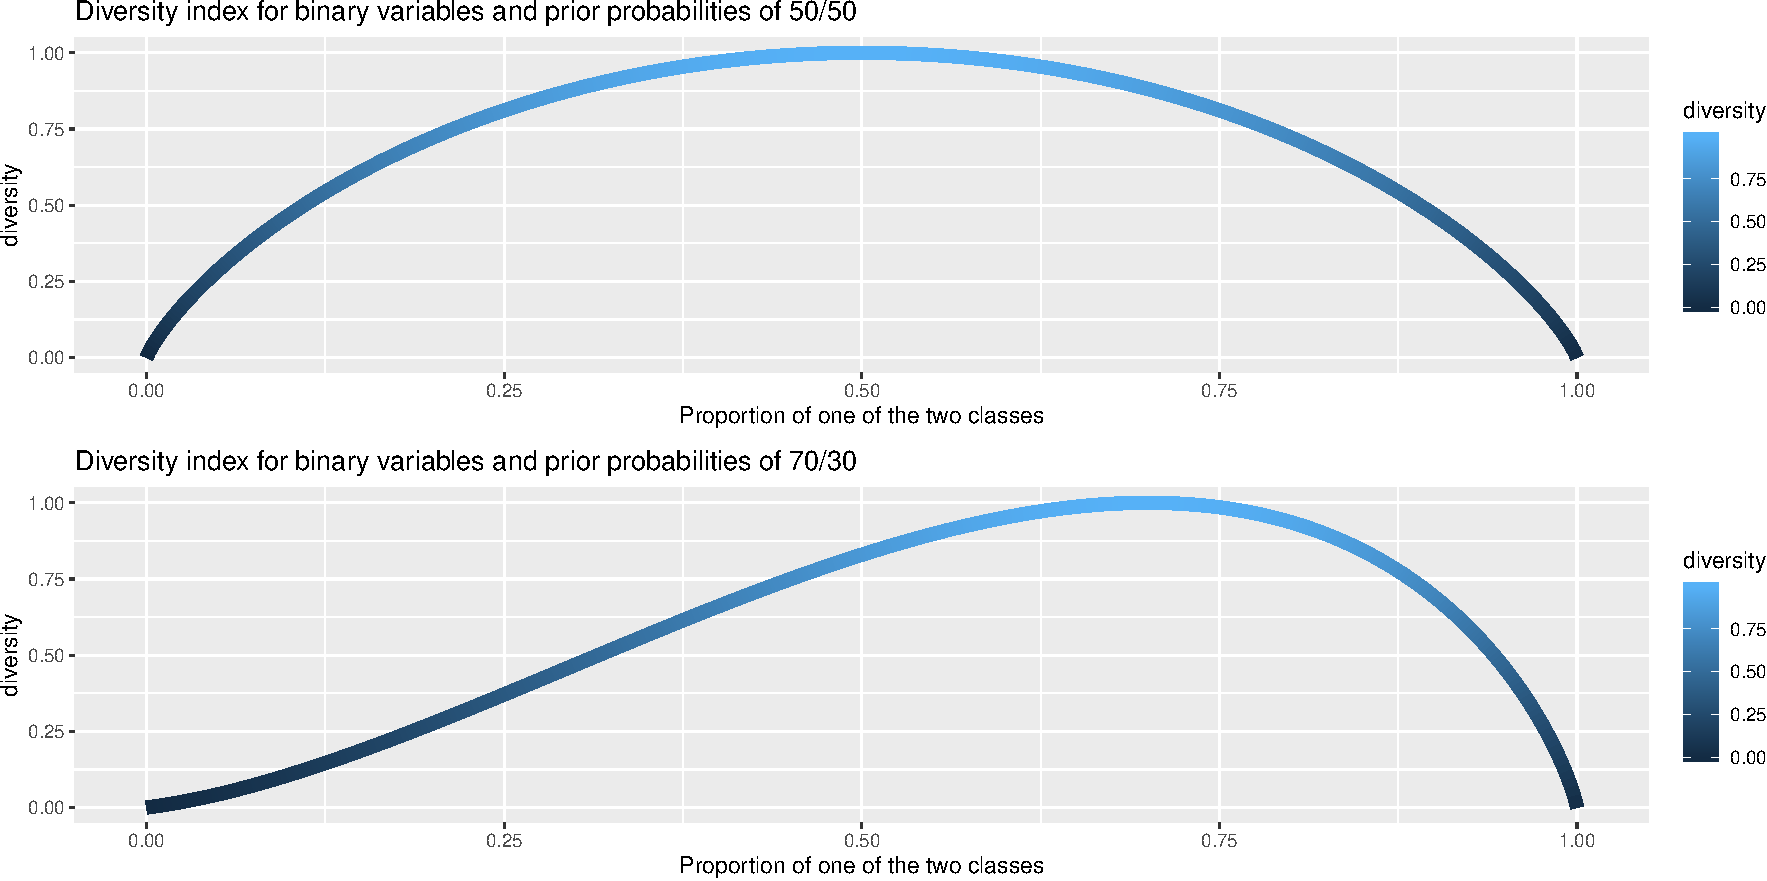
\includegraphics{team_slides_files/figure-beamer/diversityIllustrated-1.pdf}
\caption{The diversity index illustrated for the case where there are
only two possible classes, and where the prior priorities are
respectively 50/50 (top) and 70/30 (bottom). The index reaches a maximum
at a distribution equal to the prior
probabilities.\label{fig:diversityIllustrated}}
\end{figure}
\end{frame}

\begin{frame}{The confidence level and p-value}
\protect\hypertarget{the-confidence-level-and-p-value}{}
The p-value is the probability that we make a mistake by assuming that
there is no paygap.

It is calculated by splitting the data on a variable in binary factors
(e.g.~Females and others) and then checking how likely it is that a
random person from the first group earns less than a random person from
the second group. This is done by a method known as Mann-Whitney U test:
\href{https://en.wikipedia.org/wiki/Mann\%E2\%80\%93Whitney_U_test}{see
Wikipedia}\footnote<.->{The Mann--Whitney U test (aka.
  Mann--Whitney--Wilcoxon (MWW), Wilcoxon rank-sum test, or
  Wilcoxon--Mann--Whitney test) is a nonparametric test of the null
  hypothesis that, for randomly selected values X and Y from two
  populations, the probability of X being greater than Y is equal to the
  probability of Y being greater than X. If we assume that the
  distributions are symmetric, it boils down to a test that the medians
  are different.}
\end{frame}

\begin{frame}{Another view on the PayGap}
\protect\hypertarget{another-view-on-the-paygap}{}
\begin{figure}
\centering
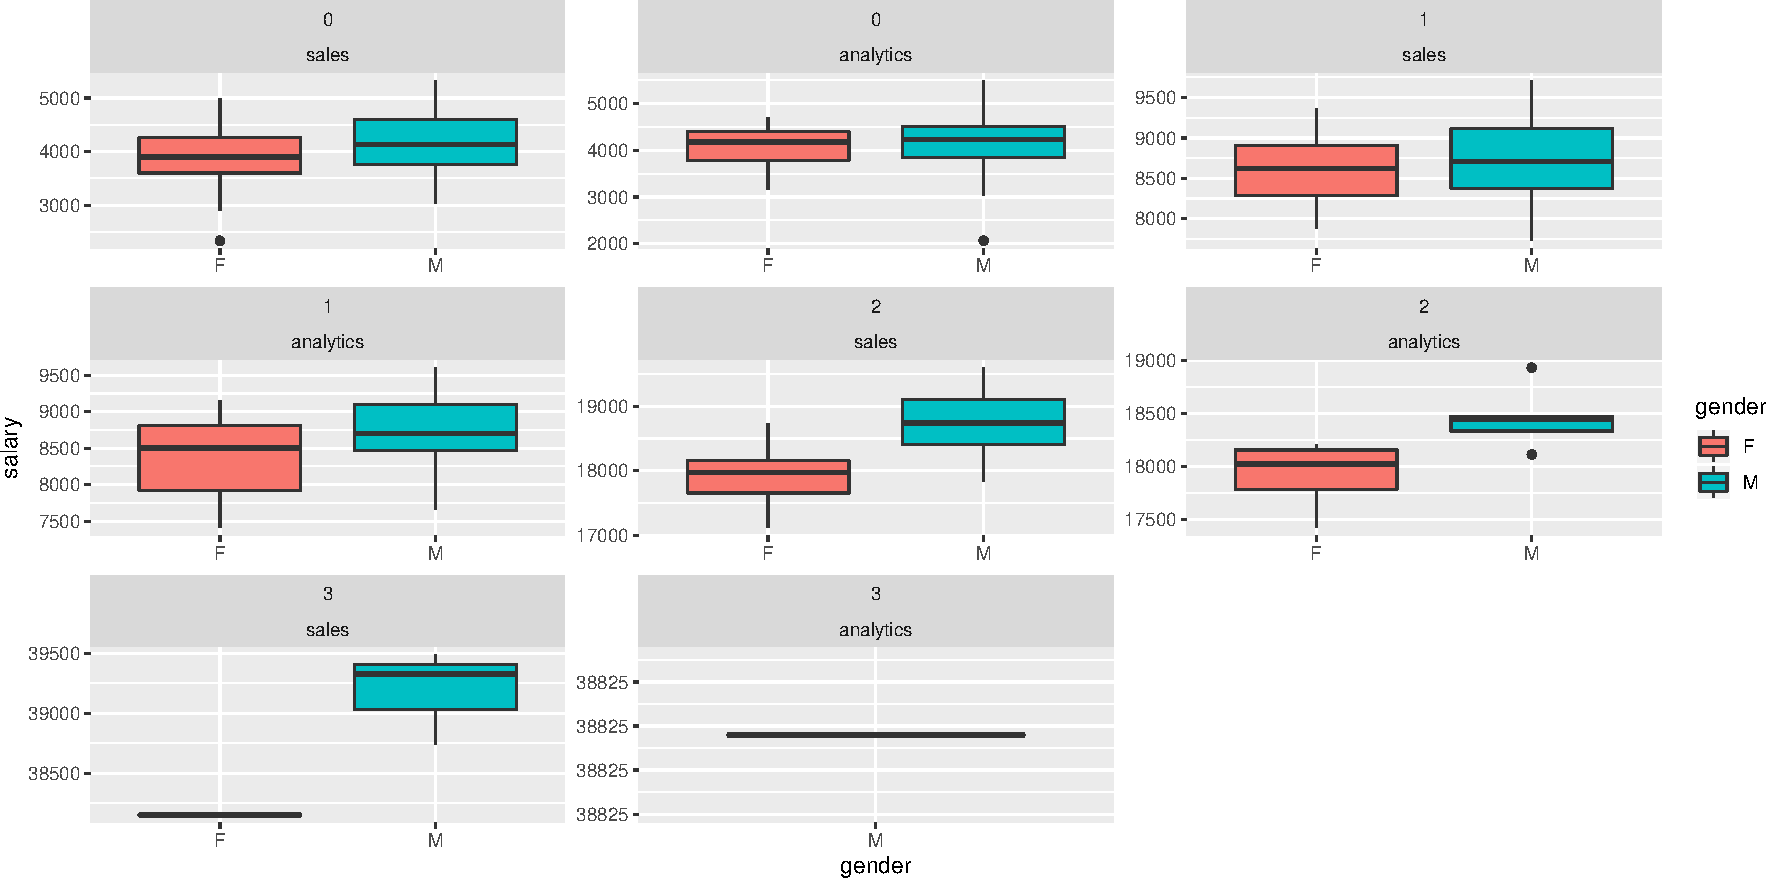
\includegraphics{team_slides_files/figure-beamer/otherPayGapGender-1.pdf}
\caption{Boxplots for each grade (over all job categories) per gender.
This another view of the same data as in Table \ref{tab:pg:gender}.}
\end{figure}
\end{frame}

\begin{frame}{Bibliography}
\protect\hypertarget{bibliography}{}
\hypertarget{refs}{}
\begin{CSLReferences}{1}{0}
\leavevmode\hypertarget{ref-debrouwer2020}{}%
De Brouwer, Philippe J.S. 2020. \emph{The Big r-Book: From Data Science
to Learning Machines and Big Data}. New York: John Wiley \& Sons, Ltd.
https://doi.org/\url{https://doi.org/10.1002/9781119632757}.

\leavevmode\hypertarget{ref-diversityhub2019}{}%
Zaroda-Dabrowska, Anna, and Tomasz Dabrowski. 2019. \emph{The Essentials
of Diversity \& Inclusion Management}. Krakow: AT Wydawnictwo.

\end{CSLReferences}
\end{frame}

\end{document}
